\subsubsection{Rancangan Detail Node}
\label{subsubsection:detail-node}

Seperti yang sudah dijelaskan pada bagian \ref{subsection:rancangan-struktural}, \textit{Node} merupakan satuan fungsional utama yang berperan sebagai entitas dalam sistem \textit{database} terdistribusi yang dikembangkan.

Struktur \textit{Node} terdiri dari:

\begin{enumerate}
    \item Subsistem penyimpanan: Subsistem ini bertanggung jawab untuk fungsionalitas \textit{key-value store} dalam sebuah \textit{Node}. Detail dari subsistem penyimpanan akan dijelaskan pada bagian \ref{subsubsection:detail-subsistem-penyimpanan}.
    \item Subsistem kontrol: Subsistem ini bertanggung jawab mengelola transaksi dan konsistensi antar-\textit{Node}. Detail dari subsistem kontrol akan dijelaskan pada bagian \ref{subsubsection:detail-subsistem-kontrol}.
    \item Komponen HTTP \textit{server}: Komponen ini berperan sebagai antarmuka komunikasi antara \textit{client} dan \textit{Node}. Detail dari komponen HTTP \textit{server} akan dijelaskan pada bagian \ref{subsubsection:detail-komponen-HTTP-server}.
    \item Komponen komunikasi antar-\textit{Node}: Komponen ini berfungsi untuk mengelola komunikasi antar-\textit{Node} dalam sistem terdistribusi. Detail dari komponen komunikasi antar-\textit{Node} akan dijelaskan pada bagian \ref{subsubsection:detail-subsistem-komunikasi-antar-node}.
\end{enumerate}

Ilustrasi struktur \textit{Node} dapat dilihat pada gambar \ref{fig:node-structure}.

% _TODO: Change image
\begin{figure}[ht]
    \centering
    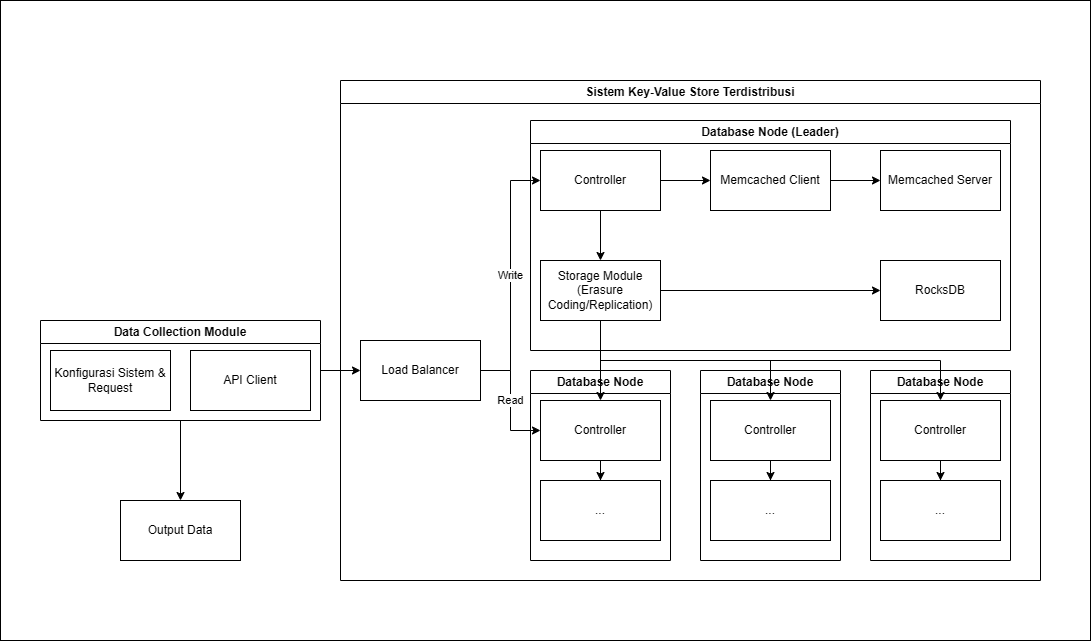
\includegraphics[width=0.95\textwidth]{resources/chapter-3/general-architecture.png}
    \caption{Struktur Node}
    \label{fig:node-structure}
\end{figure}